% Created by tikzDevice version 0.12.6 on 2025-10-29 02:04:21
% !TEX encoding = UTF-8 Unicode
\documentclass[tikz]{standalone}

\nonstopmode

\usepackage[fontset=fandol]{ctex}
\usepackage{amsfonts,bm,mathrsfs,amssymb}
\begin{document}

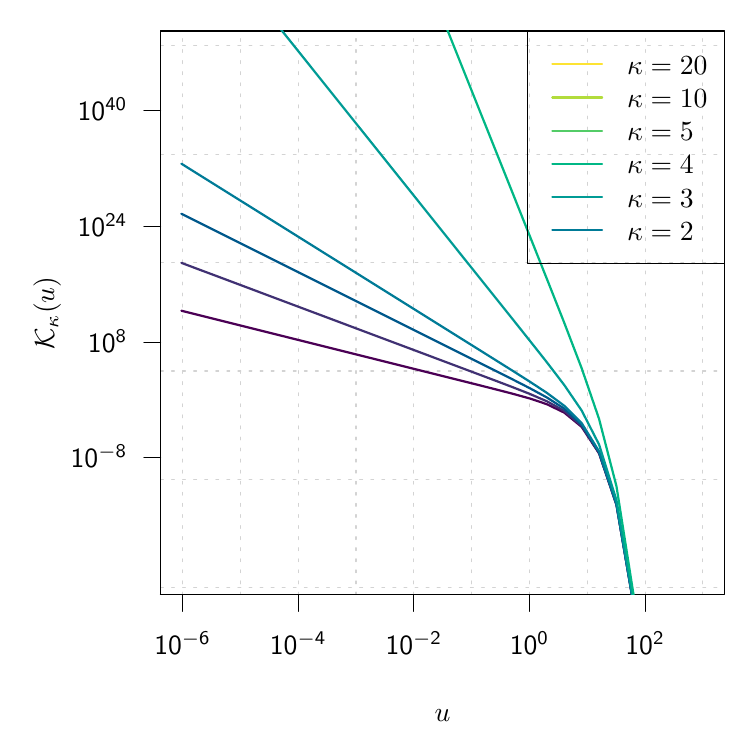
\begin{tikzpicture}[x=1pt,y=1pt]
\definecolor{fillColor}{RGB}{255,255,255}
\path[use as bounding box,fill=fillColor,fill opacity=0.00] (0,0) rectangle (252.94,252.94);
\begin{scope}
\path[clip] ( 48.00, 48.00) rectangle (251.74,251.74);
\definecolor{drawColor}{RGB}{211,211,211}

\path[draw=drawColor,line width= 0.4pt,dash pattern=on 1pt off 3pt ,line join=round,line cap=round] ( 48.00, 50.54) -- (251.74, 50.54);

\path[draw=drawColor,line width= 0.4pt,dash pattern=on 1pt off 3pt ,line join=round,line cap=round] ( 48.00, 89.71) -- (251.74, 89.71);

\path[draw=drawColor,line width= 0.4pt,dash pattern=on 1pt off 3pt ,line join=round,line cap=round] ( 48.00,128.88) -- (251.74,128.88);

\path[draw=drawColor,line width= 0.4pt,dash pattern=on 1pt off 3pt ,line join=round,line cap=round] ( 48.00,168.04) -- (251.74,168.04);

\path[draw=drawColor,line width= 0.4pt,dash pattern=on 1pt off 3pt ,line join=round,line cap=round] ( 48.00,207.21) -- (251.74,207.21);

\path[draw=drawColor,line width= 0.4pt,dash pattern=on 1pt off 3pt ,line join=round,line cap=round] ( 48.00,246.38) -- (251.74,246.38);

\path[draw=drawColor,line width= 0.4pt,dash pattern=on 1pt off 3pt ,line join=round,line cap=round] ( 55.98, 48.00) -- ( 55.98,251.74);

\path[draw=drawColor,line width= 0.4pt,dash pattern=on 1pt off 3pt ,line join=round,line cap=round] ( 76.87, 48.00) -- ( 76.87,251.74);

\path[draw=drawColor,line width= 0.4pt,dash pattern=on 1pt off 3pt ,line join=round,line cap=round] ( 97.76, 48.00) -- ( 97.76,251.74);

\path[draw=drawColor,line width= 0.4pt,dash pattern=on 1pt off 3pt ,line join=round,line cap=round] (118.65, 48.00) -- (118.65,251.74);

\path[draw=drawColor,line width= 0.4pt,dash pattern=on 1pt off 3pt ,line join=round,line cap=round] (139.54, 48.00) -- (139.54,251.74);

\path[draw=drawColor,line width= 0.4pt,dash pattern=on 1pt off 3pt ,line join=round,line cap=round] (160.42, 48.00) -- (160.42,251.74);

\path[draw=drawColor,line width= 0.4pt,dash pattern=on 1pt off 3pt ,line join=round,line cap=round] (181.31, 48.00) -- (181.31,251.74);

\path[draw=drawColor,line width= 0.4pt,dash pattern=on 1pt off 3pt ,line join=round,line cap=round] (202.20, 48.00) -- (202.20,251.74);

\path[draw=drawColor,line width= 0.4pt,dash pattern=on 1pt off 3pt ,line join=round,line cap=round] (223.09, 48.00) -- (223.09,251.74);

\path[draw=drawColor,line width= 0.4pt,dash pattern=on 1pt off 3pt ,line join=round,line cap=round] (243.98, 48.00) -- (243.98,251.74);
\end{scope}
\begin{scope}
\path[clip] (  0.00,  0.00) rectangle (252.94,252.94);
\definecolor{drawColor}{RGB}{0,0,0}

\path[draw=drawColor,line width= 0.4pt,line join=round,line cap=round] ( 48.00, 48.00) --
	(251.74, 48.00) --
	(251.74,251.74) --
	( 48.00,251.74) --
	cycle;
\end{scope}
\begin{scope}
\path[clip] (  0.00,  0.00) rectangle (252.94,252.94);
\definecolor{drawColor}{RGB}{0,0,0}

\node[text=drawColor,anchor=base,inner sep=0pt, outer sep=0pt, scale=  1.00] at (149.87,  2.40) {$u$};

\node[text=drawColor,rotate= 90.00,anchor=base,inner sep=0pt, outer sep=0pt, scale=  1.00] at (  9.60,149.87) {$\mathcal{K}_{\kappa}(u)$};
\end{scope}
\begin{scope}
\path[clip] (  0.00,  0.00) rectangle (252.94,252.94);
\definecolor{drawColor}{RGB}{0,0,0}

\path[draw=drawColor,line width= 0.4pt,line join=round,line cap=round] ( 48.00, 48.00) -- (223.09, 48.00);

\path[draw=drawColor,line width= 0.4pt,line join=round,line cap=round] ( 55.98, 48.00) -- ( 55.98, 42.00);

\path[draw=drawColor,line width= 0.4pt,line join=round,line cap=round] ( 97.76, 48.00) -- ( 97.76, 42.00);

\path[draw=drawColor,line width= 0.4pt,line join=round,line cap=round] (139.54, 48.00) -- (139.54, 42.00);

\path[draw=drawColor,line width= 0.4pt,line join=round,line cap=round] (181.31, 48.00) -- (181.31, 42.00);

\path[draw=drawColor,line width= 0.4pt,line join=round,line cap=round] (223.09, 48.00) -- (223.09, 42.00);

\node[text=drawColor,anchor=base,inner sep=0pt, outer sep=0pt, scale=  1.00] at ( 55.98, 26.40) {$\mathsf{10^{-6}}$};

\node[text=drawColor,anchor=base,inner sep=0pt, outer sep=0pt, scale=  1.00] at ( 97.76, 26.40) {$\mathsf{10^{-4}}$};

\node[text=drawColor,anchor=base,inner sep=0pt, outer sep=0pt, scale=  1.00] at (139.54, 26.40) {$\mathsf{10^{-2}}$};

\node[text=drawColor,anchor=base,inner sep=0pt, outer sep=0pt, scale=  1.00] at (181.31, 26.40) {$\mathsf{10^{0}}$};

\node[text=drawColor,anchor=base,inner sep=0pt, outer sep=0pt, scale=  1.00] at (223.09, 26.40) {$\mathsf{10^{2}}$};

\path[draw=drawColor,line width= 0.4pt,line join=round,line cap=round] ( 48.00, 97.54) -- ( 48.00,251.75);

\path[draw=drawColor,line width= 0.4pt,line join=round,line cap=round] ( 48.00, 97.54) -- ( 42.00, 97.54);

\path[draw=drawColor,line width= 0.4pt,line join=round,line cap=round] ( 48.00,139.32) -- ( 42.00,139.32);

\path[draw=drawColor,line width= 0.4pt,line join=round,line cap=round] ( 48.00,181.10) -- ( 42.00,181.10);

\path[draw=drawColor,line width= 0.4pt,line join=round,line cap=round] ( 48.00,222.88) -- ( 42.00,222.88);

\node[text=drawColor,anchor=base east,inner sep=0pt, outer sep=0pt, scale=  1.00] at ( 36.00, 93.91) {$\mathsf{10^{-8}}$};

\node[text=drawColor,anchor=base east,inner sep=0pt, outer sep=0pt, scale=  1.00] at ( 36.00,135.69) {$\mathsf{10^{8}}$};

\node[text=drawColor,anchor=base east,inner sep=0pt, outer sep=0pt, scale=  1.00] at ( 36.00,177.47) {$\mathsf{10^{24}}$};

\node[text=drawColor,anchor=base east,inner sep=0pt, outer sep=0pt, scale=  1.00] at ( 36.00,219.25) {$\mathsf{10^{40}}$};
\end{scope}
\begin{scope}
\path[clip] ( 48.00, 48.00) rectangle (251.74,251.74);
\definecolor{drawColor}{RGB}{75,0,85}

\path[draw=drawColor,line width= 0.8pt,line join=round,line cap=round] ( 55.55,150.66) --
	( 61.83,149.09) --
	( 68.12,147.51) --
	( 74.41,145.94) --
	( 80.70,144.37) --
	( 86.99,142.80) --
	( 93.28,141.23) --
	( 99.57,139.65) --
	(105.85,138.08) --
	(112.14,136.51) --
	(118.43,134.94) --
	(124.72,133.37) --
	(131.01,131.79) --
	(137.30,130.22) --
	(143.58,128.65) --
	(149.87,127.08) --
	(156.16,125.50) --
	(162.45,123.93) --
	(168.74,122.34) --
	(175.03,120.72) --
	(181.31,118.98) --
	(187.60,116.88) --
	(193.89,113.84) --
	(200.18,108.69) --
	(206.47, 99.10) --
	(212.76, 80.50) --
	(219.05, 43.78) --
	(225.33,-29.20) --
	(231.62,-174.76) --
	(237.91,-465.47);
\definecolor{drawColor}{RGB}{64,49,115}

\path[draw=drawColor,line width= 0.8pt,line join=round,line cap=round] ( 55.55,167.95) --
	( 61.83,165.59) --
	( 68.12,163.24) --
	( 74.41,160.88) --
	( 80.70,158.52) --
	( 86.99,156.16) --
	( 93.28,153.80) --
	( 99.57,151.44) --
	(105.85,149.09) --
	(112.14,146.73) --
	(118.43,144.37) --
	(124.72,142.01) --
	(131.01,139.65) --
	(137.30,137.30) --
	(143.58,134.94) --
	(149.87,132.58) --
	(156.16,130.22) --
	(162.45,127.86) --
	(168.74,125.50) --
	(175.03,123.11) --
	(181.31,120.65) --
	(187.60,117.94) --
	(193.89,114.45) --
	(200.18,109.02) --
	(206.47, 99.27) --
	(212.76, 80.58) --
	(219.05, 43.83) --
	(225.33,-29.18) --
	(231.62,-174.75) --
	(237.91,-465.47);
\definecolor{drawColor}{RGB}{0,88,139}

\path[draw=drawColor,line width= 0.8pt,line join=round,line cap=round] ( 55.55,185.70) --
	( 61.83,182.56) --
	( 68.12,179.42) --
	( 74.41,176.27) --
	( 80.70,173.13) --
	( 86.99,169.98) --
	( 93.28,166.84) --
	( 99.57,163.70) --
	(105.85,160.55) --
	(112.14,157.41) --
	(118.43,154.26) --
	(124.72,151.12) --
	(131.01,147.97) --
	(137.30,144.83) --
	(143.58,141.69) --
	(149.87,138.54) --
	(156.16,135.40) --
	(162.45,132.25) --
	(168.74,129.10) --
	(175.03,125.94) --
	(181.31,122.73) --
	(187.60,119.32) --
	(193.89,115.28) --
	(200.18,109.47) --
	(206.47, 99.51) --
	(212.76, 80.71) --
	(219.05, 43.89) --
	(225.33,-29.15) --
	(231.62,-174.74) --
	(237.91,-465.46);
\definecolor{drawColor}{RGB}{0,123,151}

\path[draw=drawColor,line width= 0.8pt,line join=round,line cap=round] ( 55.55,203.78) --
	( 61.83,199.85) --
	( 68.12,195.92) --
	( 74.41,191.99) --
	( 80.70,188.06) --
	( 86.99,184.13) --
	( 93.28,180.20) --
	( 99.57,176.27) --
	(105.85,172.34) --
	(112.14,168.41) --
	(118.43,164.48) --
	(124.72,160.55) --
	(131.01,156.62) --
	(137.30,152.69) --
	(143.58,148.76) --
	(149.87,144.83) --
	(156.16,140.90) --
	(162.45,136.97) --
	(168.74,133.03) --
	(175.03,129.09) --
	(181.31,125.11) --
	(187.60,120.98) --
	(193.89,116.31) --
	(200.18,110.05) --
	(206.47, 99.82) --
	(212.76, 80.86) --
	(219.05, 43.97) --
	(225.33,-29.11) --
	(231.62,-174.72) --
	(237.91,-465.45);
\definecolor{drawColor}{RGB}{0,155,149}

\path[draw=drawColor,line width= 0.8pt,line join=round,line cap=round] ( 55.55,297.23) --
	( 61.83,289.37) --
	( 68.12,281.51) --
	( 74.41,273.65) --
	( 80.70,265.79) --
	( 86.99,257.93) --
	( 93.28,250.07) --
	( 99.57,242.21) --
	(105.85,234.35) --
	(112.14,226.49) --
	(118.43,218.63) --
	(124.72,210.77) --
	(131.01,202.91) --
	(137.30,195.05) --
	(143.58,187.19) --
	(149.87,179.33) --
	(156.16,171.46) --
	(162.45,163.60) --
	(168.74,155.74) --
	(175.03,147.88) --
	(181.31,139.99) --
	(187.60,132.04) --
	(193.89,123.81) --
	(200.18,114.60) --
	(206.47,102.31) --
	(212.76, 82.16) --
	(219.05, 44.63) --
	(225.33,-28.78) --
	(231.62,-174.55) --
	(237.91,-465.37);
\definecolor{drawColor}{RGB}{0,183,133}

\path[draw=drawColor,line width= 0.8pt,line join=round,line cap=round] ( 55.55,492.40) --
	( 61.83,476.68) --
	( 68.12,460.96) --
	( 74.41,445.24) --
	( 80.70,429.52) --
	( 86.99,413.79) --
	( 93.28,398.07) --
	( 99.57,382.35) --
	(105.85,366.63) --
	(112.14,350.91) --
	(118.43,335.19) --
	(124.72,319.47) --
	(131.01,303.75) --
	(137.30,288.03) --
	(143.58,272.30) --
	(149.87,256.58) --
	(156.16,240.86) --
	(162.45,225.14) --
	(168.74,209.42) --
	(175.03,193.70) --
	(181.31,177.96) --
	(187.60,162.20) --
	(193.89,146.30) --
	(200.18,129.88) --
	(206.47,111.56) --
	(212.76, 87.22) --
	(219.05, 47.24) --
	(225.33,-27.46) --
	(231.62,-173.89) --
	(237.91,-465.03);
\definecolor{drawColor}{RGB}{0,0,0}

\path[draw=drawColor,line width= 0.4pt,line join=round,line cap=round] (180.58,251.74) rectangle (251.74,167.74);
\definecolor{drawColor}{RGB}{253,227,51}

\path[draw=drawColor,line width= 0.8pt,line join=round,line cap=round] (189.58,239.74) -- (207.58,239.74);
\definecolor{drawColor}{RGB}{178,220,60}

\path[draw=drawColor,line width= 0.8pt,line join=round,line cap=round] (189.58,227.74) -- (207.58,227.74);
\definecolor{drawColor}{RGB}{83,204,103}

\path[draw=drawColor,line width= 0.8pt,line join=round,line cap=round] (189.58,215.74) -- (207.58,215.74);
\definecolor{drawColor}{RGB}{0,183,133}

\path[draw=drawColor,line width= 0.8pt,line join=round,line cap=round] (189.58,203.74) -- (207.58,203.74);
\definecolor{drawColor}{RGB}{0,155,149}

\path[draw=drawColor,line width= 0.8pt,line join=round,line cap=round] (189.58,191.74) -- (207.58,191.74);
\definecolor{drawColor}{RGB}{0,123,151}

\path[draw=drawColor,line width= 0.8pt,line join=round,line cap=round] (189.58,179.74) -- (207.58,179.74);
\definecolor{drawColor}{RGB}{0,0,0}

\node[text=drawColor,anchor=base west,inner sep=0pt, outer sep=0pt, scale=  1.00] at (216.58,236.11) {$\kappa=20$};

\node[text=drawColor,anchor=base west,inner sep=0pt, outer sep=0pt, scale=  1.00] at (216.58,224.11) {$\kappa=10$};

\node[text=drawColor,anchor=base west,inner sep=0pt, outer sep=0pt, scale=  1.00] at (216.58,212.11) {$\kappa=5$};

\node[text=drawColor,anchor=base west,inner sep=0pt, outer sep=0pt, scale=  1.00] at (216.58,200.11) {$\kappa=4$};

\node[text=drawColor,anchor=base west,inner sep=0pt, outer sep=0pt, scale=  1.00] at (216.58,188.11) {$\kappa=3$};

\node[text=drawColor,anchor=base west,inner sep=0pt, outer sep=0pt, scale=  1.00] at (216.58,176.11) {$\kappa=2$};
\end{scope}
\end{tikzpicture}

\end{document}
